\subsection*{Code}
All code used to produce the results in this work was custom written in Python 3 and is publicly available online at \url{https://github.com/mptouzel/bayes_diffexpr}.

%\subsection*{Clone frequency model}
%Based on previous observations \cite{Weinstein2009,Mora2010,Mora2016e}, $\rho(f)$ is set as a power-law, i.e. $\rho(f)\propto f^{-\nu}$. The bounded domain $f_{\textrm{min}}\leq f \leq 1$ makes the proportionality factor dependent on $f_{\textrm{min}}$ and $\nu$.

%\subsection*{Noise model}
%We considered three different statistical models of cells and mRNA molecules contained in a sample. These used a negative binomial distribution, with parametrized over-dispersion: $\mathrm{NegBin}(\mu, \sigma^2=\mu+a \mu^{\gamma})$ with $a>0$ the coefficient and $\gamma>1$ the power controlling the over-dispersion, and a Poisson distribution, $\mathrm{Poisson}(\lambda)$ with scale parameter $\lambda$.
 
%The highest scoring model is of cells sampled from a negative binomial, followed mRNA molecules sampled from a Poisson distribution. A clone of size $f$ appears in a sample containing $M$ lymphocytes on average as $\mu=fM$ cells. 
%To account for over-dispersed count statistics, the number of cells is set to be Negative-Binomial distributed with mean $fM$ and variance $fM+a (fM)^{\gamma}$, with $a>0$ the coefficient and $\gamma>1$ the power controlling the over-dispersion. 
%For each clone, the number $n$ of detected mRNA molecules (i.e. UMI) is distributed according to a Poisson distribution with mean $\lambda=mN_{\textrm{reads}}/M$, where $N_{\textrm{reads}}/M$ is the average number of UMI per cell, obtained using the observed total number of molecules, $N_{\textrm{reads}}$ and $m$ is the unobserved number of cells of that clone in the sample.
  
%We inferred the parameters of this noise model, $\theta_\textrm{null}=\{f_\textrm{min},\nu,a,\gamma,M\}$, from day-0 replicates by maximizing the likelihood of the observed count pairs, $(n,n^{\prime})$, subject to the normalization constraint \ref{eq:postnorm}. The likelihood, $P(n,n^{\prime}|\theta_{\textrm{null}})$, is obtained by marginalizing over $m,m'$, and $f$.
%We implemented this constrained maximization using the scipy package implementation of the sequential least squares programming method in python.  
%$n\sim \mathrm{Poisson}(m N/M)$, $m\sim \mathrm{NegBin}(fM,fM+a (fM)^{\gamma})$, for each replicate, and $f\sim\rho$ is common to both replicates. F

\subsection*{Normalization of the clonal frequencies}\label{sec:normal}
Here we derive the condition for which the normalization in the joint density is implicitly satisfied. The normalization constant of the joint density is
\begin{equation}
	\mathcal{Z}=\int_{f_\textrm{min}}^1\cdots\int_{f_\textrm{min}}^1\prod_{i=1}^N \rho(f_i)\delta(Z-1)\textrm{d}^N\vec{f} \;\label{eq:joint},
\end{equation}
with $\delta(Z-1)$ being the only factor preventing factorization and explicit normalization. Writing the delta function in its Fourier representation factorizes the single constraint on $\vec{f}$ into $N$ Lagrange multipliers, one for each $f_i$,
\begin{align}
	\delta(Z-1)&=\int_{-i\infty}^{i\infty} \frac{\textrm{d} \mu}{2 \pi}e^{\mu(Z-1)}  \\
	&=\int_{-i\infty}^{i\infty} \frac{\textrm{d} \mu}{2 \pi}e^{-\mu}\prod_{i=1}^N e^{\mu f_i} \;.
\end{align}
Crucially, the multi-clone integral in \cref{eq:joint} over $\vec{f}$ then factorizes. Exchanging the order of the integrations we obtain
\begin{equation}
	\mathcal{Z}=\int_{-i\infty}^{i\infty} \frac{\textrm{d} \mu}{2 \pi} e^{-\mu} \langle e^{\mu f}\rangle^N\;,\label{eq:bigZ}
\end{equation}
with $\langle e^{\mu f}\rangle=\int_{f_\textrm{min}}^1\rho(f)e^{\mu f}\textrm{d}f$. Now define the large deviation function, $I(\mu):=-\frac{\mu}{N}+\log \langle e^{\mu f}\rangle$, so that 
\begin{equation}
	\mathcal{Z}=\int_{-i\infty}^{i\infty} \frac{\textrm{d} \mu}{2 \pi} e^{-N I(\mu)}\;.\label{eq:largedev}
\end{equation}
Note that $I(0)=0$. With $N$ large, this integral is well-approximated by the integrand's value at its saddle point, located at $\mu^*$ satisfying $I'(\mu^*)=0$.  Evaluating the latter gives
\begin{align}
	\frac{1}{N}&=\frac{\langle f e^{\mu^* f}\rangle}{\langle e^{\mu^* f}\rangle}\;.
\end{align} 
If the left-hand side is equal to $\langle f\rangle$, the equality holds only for $\mu^*=0$ since expectations of products of correlated random variables are not generally products of their expectations. 
In this case, we see from \cref{eq:largedev} that $\mathcal{Z}=1$, and so the constraint $N\langle f\rangle=1$ imposes normalization.
% \begin{align}
% 	\langle g(\vec{f})\rangle_{\rho_N(\vec{f})}&=\int_{f_\textrm{min}}^1\cdots\int_{f_\textrm{min}}^1\prod_{i=1}^N \rho(f)\frac{1}{2 \pi} \int_{-i\infty}^{i\infty} e^{i \mu(Z-1)} \textrm{d} \mu \textrm{d}^N\vec{f} g(\vec{f})\\
% 	\int_{f_\textrm{min}}^1\cdots\int_{f_\textrm{min}}^1\prod_{i=1}^N \rho(f)\frac{1}{2 \pi} \int_{-i\infty}^{i\infty} e^{i \mu(Z-1)} \textrm{d} \mu \textrm{d}^N\vec{f} g(\vec{f})\;.
% \end{align}

\subsection*{Null model sampling}\label{sec:null_sampling}
The procedure for null model sampling is summarized as (1) fix main model parameters, (2) solve for remaining parameters using the normalization constraint, $N \langle f \rangle=1$, and (3) starting with frequencies, sample and use to specify the distribution of the next random variable in the chain.

In detail, we first fix: (a)
%\begin{itemize}
%\item
the model parameters $\{\alpha,M,a,\gamma\}$, excluding $f_{\textrm{min}}$;
% Separate $M$, $a$, and $\gamma$ values could be defined for the reference and test condition, respectively. The empirical $P(n,n^{\prime})$ for replicate data was found to be highly symmetric in $n$ and $n^{\prime}$ across donors, however, supporting the assumption of a single acquisition model and so we neglect this complication. 
% \item
(b) the desired size of the full repertoire, $N$;
%Together with the model prediction of capture efficiency, $1-P(0,0)$, this gives the number of clones we should sample, $N_{\textrm{\textrm{obs}}}$, via $N_{\textrm{\textrm{obs}}}=N(1-P(0,0))$, 
% \item
(c) the sequencing efficiency (total sample reads/total sample cells), $\epsilon$. From this we get the effective total sample reads, $N^{\textrm{eff}}_{\textrm{reads}}=\epsilon M$, which converts a clone's frequency to the average number of cells it appears with in the sample.
% (We could in fact define two sequencing efficiencies, one for each replicate, leading to different effective total number of reads in each replicate).
Note that the actual sampled number of reads is stochastic and so will differ from this fixed value.
%\end{itemize}

We then solve for remaining parameters. Specifically, $f_{\textrm{min}}$ is fixed by the constraint that the average sum of all frequencies, under the assumption that their distribution factorizes, is unity:
\begin{equation}
% 	P(0,0)N\langle f\rangle_{\rho(f|n+n^{\prime}=0)} + N_{\textrm{\textrm{obs}}} \langle f\rangle_{\rho(f|n+n^{\prime}>0)} = 1
	N \langle f\rangle_{\rho(f)}=1
\end{equation}
This completes the parameter specification.

We then sample from the corresponding chain of random variables.
Sampling the chain of random variables of the null model can be performed efficiently by only sampling the $N_{\textrm{obs}}=N(1-P(0,0))$ observed clones. This is done separately for each replicate, once conditioned on whether or not the other count is zero. 
Samples with 0 molecule counts can in principle be produced with any number of cells, so cell counts must be marginalized when implementing this constraint. We thus used the conditional probability distributions $P(n|f)=\sum_{m}P(n|m)P(m|f)$ with $m,n=0,1,\dots$. $P(n^\prime|f)$ is defined similarly. Note that these two conditional distributions differ only in their average number of UMI per cell, $N_{\textrm{read}}/M$, due to their differing number of observed total number of molecules, $N_{\textrm{read}}$. Together with $\rho(f)$, these distributions form the full joint distribution, which is conditioned on the clone appearing in the sample, i.e. $n+n^{\prime}>0$ (denoted $\mathcal{O}$), 
\begin{align}
	P(n,n^{\prime},f|\mathcal{O})= \frac{P(n|f)P(n^{\prime}|f)\rho(f)}{1-\int{\textrm{d}f \rho(f)\textrm{d}f P(n=0|f)P(n^{\prime}=0|f)}}\;,  
\end{align}
with the renormalization accounting for the fact that $(n,n^{\prime})=(0,0)$ is excluded. The 3 quadrants having a finite count for at least one replicate are denoted $q_{x0}$, $q_{0x}$, and $q_{xx}$, respectively. Their respective weights are
\begin{align}
	P(q_{x0}|\mathcal{O})&=&\sum_{n>0}\int{\textrm{d}f P(n,n^{\prime}=0,f|\mathcal{O})}\;,\\
	P(q_{0x}|\mathcal{O})&=&\sum_{n^{\prime}>0}\int{\textrm{d}f P(n=0,n^{\prime},f|\mathcal{O})}\;,\\
	P(q_{xx}|\mathcal{O})&=&\sum_{\substack{n>0,\\n^{\prime}>0}}\int{\textrm{d}f P(n,n^{\prime},f|\mathcal{O})}.
\end{align}
Conditioning on $\mathcal{O}$ ensures normalization, $P(q_{x0}|\mathcal{O})+P(q_{0x}|\mathcal{O})+P(q_{xx}|\mathcal{O})=1$. Each sampled clone falls in one the three regions according to these probabilities. Their clone frequencies are then drawn conditioned on the respective region, 
\begin{align}
	P(f|q_{x0})&=&\sum_{n>0}P(n,n^{\prime}=0,f|\mathcal{O})/P(q_{x0}|\mathcal{O})\;,\\
	P(f|q_{0x})&=&\sum_{n^{\prime}>0}P(n=0,n^{\prime},f|\mathcal{O})/P(q_{0x}|\mathcal{O})\;,\\
	P(f|q_{xx})&=&\sum_{{n>0,n^{\prime}>0}}P(n,n^{\prime},f|\mathcal{O})/P(q_{xx}|\mathcal{O}).
\end{align}

Using the sampled frequency, a pair of molecule counts for the three quadrants are then sampled as $(n,0)$, $(0,n^{\prime})$, and $(n,n^{\prime})$, respectively, with $n$ and $n^{\prime}$ drawn from the renormalized, finite-count domain of the conditional distributions, $P(n|f,n>0)$. 

% Using the sampled frequency, a pair of number of cells $(m,m^{\prime})$ is obtained. For $q_{x0}$, $m$ is sampled from $P(m|f,n>0)$ and $m^{\prime}$ sampled from $P(m^{\prime}|f,n^{\prime}=0)$ with 
% \begin{align}
% 	P(m|f,n>0)&=&\frac{\sum_{n>0}P(m,n|f)}{\sum_{\substack{n>0,\\m}}P(m,n|f)}\;,\\
% 	P(m^{\prime}|f,n^{\prime}=0)&=&\frac{P(m^{\prime},n^{\prime}=0|f)}{\sum_{m^{\prime}}P(m^{\prime},n^{\prime}=0|f)}\;,
% \end{align}
% with $P(m_i,n_i|f)=P(n_i|m_i)P(m_i|f)$, for $i=1,2$. Note that by construction here, $m>0$, since $P(n>0|m=0)=0$.
% The procedure is similar for frequencies sampled in $q_{0x}$. For frequencies sampled in $q_{xx}$, cell count pairs $(m,m^{\prime})$ are sampled from $P(m|f,n>0)$ and $P(m^{\prime}|f,n^{\prime}>0)$, respectively. 
% 
% Molecule counts for the three quadrants are then sampled as $(n,0)$, $(0,n^{\prime})$, and $(n,n^{\prime})$, respectively, with $n$ and $n^{\prime}$ drawn from the renormalized, finite-count domain of the conditional distributions, $P(n|m)$ and $P(n^{\prime}|m^{\prime})$, respectively, with $m>0$ and $m^{\prime}>0$. 

Using this sampling procedure we demonstrate the validity of the null model and its inference by sampling across the observed range of parameters and reinferring their values (see \cref{fig:SM_reinfer_null}).


\subsection*{Differential model sampling}\label{sec:diffexpr_sampling}
Since the differential expression model involves expansion and contraction in the test condition, some normalization in this condition is needed such that it produces roughly the same total number of cells as those in the reference condition, consistent with the observed data. One approach (the one taken below) is to normalize at the level of clone frequencies. 
Here, we instead perform the inefficient but more straightforward procedure of sampling all $N$ clones and discarding those clones for which $(n,n^{\prime})=(0,0)$. A slight difference in the two procedures is that $N_{\textrm{obs}}$ is fixed in the former, while is stochastic in the latter.


%\subsection*{Direct sampling}
The frequencies of the first condition, $f_i$, are sampled from $\rho(f)$ until they sum to 1 (i.e. until before they surpass 1, with a final frequency added that takes the sum exactly to 1). An equal number of log-frequency fold-changes, $s_i$, are sampled from $\rho(s)$. The normalized frequencies of the second condition are then $f'_i=f_ie^{s_i}/\sum_j f_je^{s_j}$.  Counts from the two conditions are then sampled from $P(n|f)$ and $P(n^{\prime}|f')$, respectively. Unobserved clones, i.e. those with $(n,n^{\prime})=(0,0)$, are then discarded.

% \subsubsection*{Effective sampling}
% For an efficient implementation, the procedure should avoid sampling the numerous clones that produce $(n,n^{\prime})=(0,0)$, since these are discarded. Such a procedure follows. 
% 
% First, the $(f,s)$-plane is partitioned into two regions, $D=\{(f,s)|f<f_0,fe^s<f_0\}$ and its complement, $\bar D$, with $f_0$ chosen such that clones sampled from $\bar D$ are often \textit{observed}, i.e. $n+n^{\prime}>0$ (a minority of clones sampled in $\bar D$ will nevertheless give $n+n^{\prime}=0$; these are discarded). In contrast, frequencies sampled from $D$ will be small, so that most will be unobserved, and we must condition on the clone being observed when sampling from this regime. Moreover, their average is unaffected by the long-tailed behaviour of the distribution in the large-frequency regime and thus is well-approximated by the corresponding ensemble average. We use this latter fact when computing the renormalization of the frequencies of the second condition. 
% 
% We compute the mass in $D$ as $P_D=\int_f \textrm{d}f\rho(f)\sum_s \rho(s) \mathbb{1}((f,s)\in D)$.
% 
% We sample $(f,s)$ in $\bar D$ until the sum of the first condition^{\prime}s frequencies, $\sum_i f_i$ added to the expected sum in $D$, $P_D N_{cl}\langle f\rangle_{P(f|D)}$, equals 1,
% \begin{align}
% 	1=\sum_{i=1}^{N_{\bar D}} f_i + P_D N_{cl}\langle f\rangle_{P(f|D)}\;,
% \end{align}
% where $N_{cl}$ is the total number of clones in the repertoire. The number sampled from $\bar D$, $N_{\bar D}$, is determined from that expression self-consistently by substituting $N_{cl}=N_{\bar D}/(1-P_D)$ obtained from $N_{\bar D}+P_D N_{cl}\equiv N_{cl}$. The normalization for the second condition^{\prime}s frequencies is then 
% \begin{align}
% 	Z=\sum_{i=1}^{N_{\bar D}} f_ie^{s_i} + P_D N_{cl}\langle fe^s\rangle_{P(f,s|D)}
% \end{align}
% such that the second condition^{\prime}s frequencies are ${f_i'=f_ie^{s_i}/Z}$. Molecule counts are then sampled from $P(n|f)$ and $P(n^{\prime}|f')$.  
% 
% We then sample from $D$ conditioned on the clone being observed, i.e. having produced a finite number of molecules in either of the two conditions. We thus sample $N_D=P(n+n^{\prime}>0|D)P_D N_{cl}$ clones from $P(f,s|D,n+n^{\prime}>0)$. To avoid having to sample over the joint distribution of $n$ and $n^{\prime}$, we condition on the 3 regions of finite counts in both conditions, $(n,0)$, $(0,n^{\prime})$, and $(n,n^{\prime})$, in which $n$ and $n^{\prime}$ can be sampled independently. 
% Note the presence of the normalization factor, $Z$, in 
% \begin{align}
% 	P(n+n^{\prime}>0|D)=\int_f \textrm{d}f\rho(f)\sum_s \rho(s)(1-P(n=0|f)P(n^{\prime}=0|f'=fe^s/Z))\;.
% \end{align}
% and
% \begin{align}
% 	P(f,s|D,n+n^{\prime}>0)=\frac{\rho(f)\rho(s)(1-P(n=0|f)P(n^{\prime}=0|f'=fe^s/Z))}{P(n+n^{\prime}>0|D)P_D}\;.
% \end{align}
% We then concatenate the $N_D$ sampled counts from $D$ and the $N_{\bar D}$ sampled counts (with $(n,n^{\prime})=(0,0)$ realizations discarded) from $\bar D$ to obtain the full data set.  

% \subsection*{Null Model Inference}
% Given a data set, $\mathcal{D}=\{(n_i,n^{\prime}_i)\}_{i=1}^{N_{\textrm{obs}}}$, we infer the parameters of the null model, $\Theta_{\textrm{null}}=(\alpha,a,\gamma,M,f_{\textrm{min}})$ by maximizing the marginal likelihood of the observable model, $P(n,n^{\prime}|n+n^{\prime}>0,\Theta_{\textrm{null}})$, subject to the normalization constraint$, N\langle f\rangle_{\rho(f)}=1$, where $N=N_{\textrm{obs}}/(1-P(0,0))$. Since in this case we have access to a realization, we could instead normalize conditioned on this realization. Since, 
% \begin{equation*}
% 	N\sum_{(n,n^{\prime})>0}P(n,n^{\prime})\approx N\sum_{(n,n^{\prime})\in \mathcal{D}}\frac{\#(n,n^{\prime})}{N}\equiv \sum_{i}^{N_{\textrm{obs}}}
% \end{equation*}
% we then have
% \begin{equation}
% 	1=N\langle f\rangle_{\rho(f|\mathcal{D})}
% 							   = P(0,0)N\langle f\rangle_{\rho(f|n+n^{\prime}=0)} + \sum_{i}^{N_{\textrm{obs}}}\langle f\rangle_{\rho(f|n_i,n^{\prime}_i)}\;.
% \end{equation}

% \subsection*{Differential expression model definition}
% We introduce a selection factor $s$ defined as the log-frequency fold-change between a clone's frequency on one day, $f$, and that on another, $fe^s$, and define $P(n,n^{\prime}|s,\theta_n)$ as before, but replacing $f$ by $fe^s$ in the definition of $m^{\prime}$. Given a prior distribution  $P(s|\theta_s)$ over $s$ parametrized by a set of parameters $\theta_s$ distinct from $\theta_n$, we used Bayes rule to obtain the posterior log-frequency fold-change probability function given an observed count pair, $P(s|n,n^{\prime},\theta_n,\theta_s)$. We set the values of the parameters $\theta_s$ of this prior by again maximizing the likelihood of the count pair data given the model over $\theta_s$, $\int P(n,n^{\prime}|s,\theta_n)P(s|\theta_s)\textrm{d}s$.
% 
% We explored a family of priors expressible as 
% \begin{eqnarray}
% 	P(s|\theta_s)&=&\frac{\alpha \beta}{Z_+}e^{-\frac{|s-s_0|}{s_+}}\Theta(s-s_0) \nonumber\\
% 	&&+\frac{\alpha (1-\beta)}{Z_-}e^{-\frac{|s-s_0|}{s_-}}\Theta(s_0-s) \\
% 	&&+(1-\alpha)\delta(s-s_0)\;, \label{eq:genPs}\nonumber
% \end{eqnarray}
% with $Z_{\pm} \sim s_{\pm}$ (see  \cref{fig:Ps}) so that in the most general prior, $\theta_s=(s_-,s_+,\alpha,\beta,s_0)$. See table \ref{Tbl1:Priors} for reduced-parameter versions of this model that we considered.


\subsection*{Obtaining diversity estimates from the clone frequency density}\label{sec:infer_div}
For a set of clone frequencies, $\{f_i\}_{i=1}^{N}$, the Hill family of diversities are obtained from the R\'enyi entropies, as $D_\beta=\exp H_\beta$, with $H_\beta=\frac{1}{1-\beta}\ln \left[ \sum_{i=1}^N f_i^{\beta}\right]$. We use $\rho(f)$ to compute their ensemble averages over $f$, again under the assumption that the joint distribution of frequencies factorizes. We obtain an estimate for $D_0=N$ using the model-derived expression, $N_{\textrm{obs}}+P(n=0)N=N$, where $N_{\textrm{obs}}$ is the number of clones observed in one sample, and $P(n=0)=\int_{f_{\textrm{min}}}^1 P(n=0|f)\rho(f)\textrm{d}f$. For $\beta=1$, we compute $\exp (N\langle -f\log f \rangle_{\rho(f)})$ and for $\beta=2$, we use $1/\left(N\langle f^2\rangle_{\rho(f)}\right)$.


% \begin{align}
% 	P(f,s|n,n^{\prime})&=&\frac{P(n,n^{\prime},f,s)}{\int\textrm{d}f\int\textrm{d}s P(n,n^{\prime},f,s)}
% \end{align}
% and using this, $P(f|n+n^{\prime}>0)=\int\textrm{d}s P(f,s|n,n^{\prime})$. 
% 
% \re{need to mention that the realization specific constraints are used here.}
% 
% The shift enters in $P(n,n^{\prime},f,s)=P(n|f)P(n^{\prime}|f,s)\rho(f)\rho_{s_0}(s)$ via $\rho_{s_0}(s)$. A convenient change of variables $s\leftarrow\Delta s+s_0$ maps $\rho_{s_0}(s)$ to $\rho_{0}(\Delta s)$, upon which
% \begin{align}
% 	\langle fe^s \rangle &=&\int{ \textrm{d}f \sum_{\Delta s} fe^{\Delta s+s_0} P(n|f)P(n^{\prime}|f,\Delta s+s_0)\rho(f)\rho_{0}(\Delta s)} \\
% 						 &=&e^{s_0}\int{ \textrm{d}f \sum_{\Delta s} fe^{\Delta s} P(n|f)P(n^{\prime}|f,\Delta s+s_0)\rho(f)\rho_{0}(\Delta s)}\;.
% \end{align}
% Denoting the remaining integral, $\tilde{\langle fe^s \rangle}$, and performing the same change of variables on $\langle f \rangle$,
% \begin{align}
% 	\langle f \rangle &=&\int{ \textrm{d}f \sum_{\Delta s} f             P(n|f)P(n^{\prime}|f,\Delta s+s_0)\rho(f)\rho_{0}(\Delta s)}\;,
% \end{align}
% the condition can be written as $s_0=\ln \tilde{\langle fe^s \rangle} - \ln \langle f \rangle$. To obtain $s_0$ from this implicit equation, we apply an iterative scheme beginning with $s_0=0$. We compute $P(n^{\prime}|f,\Delta s+s_0)$, and then the latter expression supplies $s_0$ in the next iteration. In practice, we take a bounded range of $\Delta s$ symmetric around 0. Thus, the only factor containing shift information is $P(n^{\prime}|f,\Delta s+s_0)$ appearing in both $\tilde{\langle fe^s \rangle}$ and $\langle f \rangle$. However, for self-consistent numerics, the $e^{\Delta s}$ factor must be defined over a shifted domain.

\subsection*{Inferring the differential expression prior}\label{sec:EM}
To learn the parameters of $\rho(s)$, we performed a grid search, refined by an iterative, gradient-based search to obtain the maximum likelihood.

In a more formal approach, here we employ expectation maximization (EM) to obtain the optimal parameter estimates from the data by calculating the expected log likelihood over the posterior and then maximizing with respect to the parameters. In practice, we first perform the latter analytically and then evaluate the former numerically. We choose a symmetric exponential as a tractable prior for this purpose:
\begin{align}
	\rho_{\rm exp}(s|\bar{s})=e^{-|s|/\bar{s}}/2\bar{s}
\end{align}
with $\bar{s}>0$, and no shift, $s_0=0$. The expected value of the log likelihood function, often called the Q-function in EM literature, is 
 \begin{align}
 Q(\bar{s}|\bar{s}')=\sum_{i=1}^{N_\textrm{\textrm{obs}}}\int_{-\infty}^{\infty}\mathrm{d}s\rho(s|n_i,n_i^{\prime},\bar{s}')\log \left[P(n_i,n_i^{\prime},s|\bar{s})\right]\;,
 \end{align}
 where $\bar{s}'$ is the current estimate.
 Maximizing $Q$  with respect to $\bar{s}$ is relatively simple since $\bar{s}$ appears only in $\rho_{\rm exp}(s|\bar{s})$  which is a factor in $P(n,n^{\prime},s|\bar{s})$. For each $s$,
 \begin{align}
 \frac{\partial \log \left[\rho_{\rm exp}(s|\bar{s}))\right] }{\partial\bar{s}} &=\frac{1}{\rho_{\rm exp}(s|\bar{s})} \frac{\partial\rho_{\rm exp}(s|\bar{s})}{\partial\bar{s}}\\&=\frac{|s|-\bar{s}}{\bar{s}^2}\;,
 \end{align}
so that $  \frac{\partial Q(\bar{s}|\bar{s}')}{\partial\bar{s}}=\sum_{i=1}^{N_\textrm{obs}}\int_{-\infty}^{\infty}\mathrm{d}s\rho(s|n_i,n_i^{\prime},\bar{s}')\frac{\partial \log \left[\rho_{\rm exp}(s|\bar{s}))\right] }{\partial\bar{s}} =0$ implies
\begin{align}
  \sum_{i=1}^{N_\textrm{obs}}\int_{-\infty}^{\infty}\mathrm{d}s\rho(s|n_i,n_i^{\prime},\bar{s}')\frac{|s|-\bar{s}^*}{\bar{s}^{*2}} =0
\end{align}
so that $\bar{s}^*=\frac{1}{N_\textrm{\textrm{obs}}}\sum_{i=1}^{N_\textrm{obs}}\bar{s}_{(n_i,n_i^{\prime})}$, where 
\begin{align}
\bar{s}_{(n,n^{\prime})}=\int_{-\infty}^{\infty}\mathrm{d}s|s|\rho(s|n,n^{\prime},\bar{s}').
\end{align}
The latter integral is computed numerically from the model using $\rho(s|n,n^{\prime},\bar{s}')=P(n,n^{\prime},s|\bar{s}')/\int_{-\infty}^{\infty}P(n,n^{\prime},s|\bar{s}')\mathrm{d}s	$. $Q$ is maximized at $\bar{s}=\bar{s}^*$ since  $ \frac{\partial^2 \log \left[\rho_{\rm exp}(s|\bar{s}))\right] }{\partial\bar{s}^2}\bigg|_{\bar{s}=\bar{s}^*}=-\bar{s}^{*-2} <0$. Thus, we update $\rho_{\rm exp}(s|\bar{s})$ with 
$\bar s\leftarrow\bar{s}^*$.
The number of updates typically required for convergence was small.

%\subsection*{Deriving update for shift, $s_0$} \label{sec:shift_proc}
The constraint of equal repertoire size, $Z^\prime=Z$ can be satisfied with a suitable choice of the shift parameter, $s_0$, in the prior for differential expression, $\rho_{s}(s)$, namely $s_0=-\ln Z^\prime/Z$. The latter arises from the coordinate transformation $s\leftarrow\Delta s+s_0$ that maps $\rho_{s_0}(s)$ to $\rho_{0}(\Delta s)$, and adds a factor of $e^{s_0}$ to all terms of $Z^\prime$.


%\subsection*{Identifying responding clones}
%In analogy with $p$-values, we used the posterior probability corresponding to the null hypothesis that they are not expanded, $p=\rho(s\leq 0|n,n^{\prime},\theta_{\rm null},\theta_{\rm exp})$ to rank the clones by the significance of their expansion, using a threshold of $p<0.025$. 



%\lange fe^s \rangle &=&\int{ \textrm{d}f \sum_s fe^s p(f|n+n^{\prime}>0)}\;,

% Candidate responding clones were identified using a model of RNA count statistics accounting for differential expression and the sequencing process. A full presentation will be published elsewhere. Here, we provide a brief exposition of the model and how we have applied it. The core repertoire object in the model is a probability density function, $\rho(f)$, of normalized clone size, called clone frequency, $f\in[1/m_{total},1]$, where $m_{total}=10^{11}$ is an estimate of the total number of lymphocytes in an individual. $\rho(f)\mathrm{d}f$ is then the probability that a randomly sampled clone takes up a fraction $f$ of the repertoire. We set $\rho(f)\propto f^{\gamma}$, i.e. power-law distributed with the power $\gamma<0$, consistent with many observed unpartitioned sampled repertoires.
% 
% Next, a blood sample contains a sampled repertoire in the form of an a priori unknown number of lymphocytes, $m_{sample}$. Across many clones of size $f$ in the sample, these will appear on average with $\bar{m}(f)=fm_{sample}$ cells. In our data and elsewhere, prevalent overdispersion is observed in the count statistics. We thus employ the mean-variance relation, $\sigma_m^2(f)=\bar{m}(f)+a \bar{m}(f)^{\beta}$, with $a>0$ the coefficient and $\beta>1$ the power controlling the over-dispersion. We set the number of cells to be Negative-Binomial distributed with mean $\bar{m}(f)$ and variance $\sigma_m^2$. 
% 
% Finally, the cells in the sample are then barcode-sequenced, resulting in a number of putative RNA molecules, $n$, for each clone. $m$ cells will produce $\bar{n}(m)=mr_c$ molecules on average where $r_c>0$ is the average number of RNA molecules per cell. $r_c$ brings together into a single parameter a variety of diluting effects, heterogeneous across samples so that we expect $r_c<1$. For an total observed number of observed reads, $n_{sample}$, $r_c$ is related to $m_{sample}$ via $n_{sample}=r_cm_{sample}$. Even though $m_{sample}$ is precisely controlled by the sampled volume, $n_{sample}$ still varies due to procedural variation in sequencing. Thus, we let $r_c$ account for this variation by setting it as $r_c=m_{sample}/n_{sample}$. We set the number of molecules to be Poisson-distributed with scale parameter $\bar{n}(f)$.
% 
% We used day-0 replicates to infer maximum likelihood estimates for these parameters using the likelihood function,
% \begin{align}
% \mathcal{L}(\gamma,m_{sample},a,\beta)=\frac{1}{N_{clones}}\sum_{(n,n^{\prime})_{data}}\log P_{\mathrm{same}}(n,n^{\prime})
% \end{align}
% where $N_{clones}$ is the number of observed clones and
% \begin{align}
% P_{\mathrm{same}}(n,n^{\prime})&=\int_{1/m_{total}}^1P(n|f=f)P(n^{\prime}|f^{\prime}=f)\rho(f)\mathrm{d}f\\
% P(n|f)&=\sum_{m=0}^{\infty}\mathcal{NB}_{\bar{m}(f),\sigma^2_{m}(f)}(m)Pois_{\bar{n}(m)}(n)\;.
% \end{align}
% This fitted model characterizes the variation expected of pairs of sampled repertoires for unchanged antigen conditions.
% 
% For changing antigen conditions, the clone frequencies making up the repertoire will change. Using $s$ to denote the log-frequency fold-change between a clone's frequency in one condition, $f$, and another $f^{\prime}=fe^s$, a distribution of these changes, $\rho(s)$, exists. A particular $\rho(s)$ serves as a prior distribution for these changes. The posterior probability given an observed count pair is then
% \begin{align}
% P(s|n,n^{\prime})\propto P(n,n^{\prime}|s)\rho(s)
% \end{align}
% where 
% \begin{align}
% P(n,n^{\prime}|s)=\int_{1/m_{total}}^1P(n|f=f)P(n^{\prime}|f^{\prime}=fe^s)\rho(f)\mathrm{d}f\;.
% \end{align}
% Note the additional factor of $e^s$ compared with the same-day model in the expression for $f^{\prime}$. 
% The posterior distribution of fold change given an observed count pair can be used to rank the clones by the significance of their expansion. In analogy with p-values, we use the posterior probability corresponding to the null hypothesis that they are not expanded, $P(s\leq 0|n,n^{\prime})$ and set a threshold of significance $P(s\leq 0|n,n^{\prime})\leq 0.025$. 
% 
% We parametrize our prior, $\rho(s)$, with  $\alpha\in[0,1]$, the fraction of clones that responds to the change, and $\bar{s}>0$, their typical effect size. Accordingly, we set $\rho(s)=\frac{\alpha}{Z}\exp\left[-|s|/\bar{s}\right]+(1-\alpha)\delta(s)$, where the normalization, $Z$, is such that the first term integrates to $\alpha$. We set the values of the parameters of this prior by again maximizing the likelihood of the data given the corresponding model,
% \begin{align}
% \mathcal{L}(\alpha,\bar{s})=\frac{1}{N_{clones}}\sum_{(n,n^{\prime})_{data}}\log P_{\mathrm{diff}}(n,n^{\prime})
% \end{align}
% where
% \begin{align}
% P_{\mathrm{diff}}(n,n^{\prime})=\int_{s_{min}}^{s_{max}}P(n,n^{\prime}|s)\rho(s)\mathrm{d}s\;.
% \end{align}



	
%An asymmetric exponential decay away from a shifted center at which a non-responding fraction is placed (see  \cref{eq:genPs} and  \cref{fig:Ps}).

% \begin{figure}[h!]
% 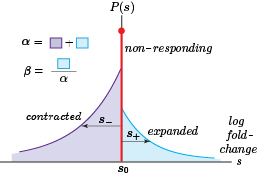
\includegraphics{schematic}
% \centering{}
% \caption{
% \emph{Functional forms of prior on clone size log-frequency fold-change}. $\rho(s)$,  \cref{eq:genPs}, is parametrized most generally here by an effect size for both expansion, $s_+$, and contraction,$s_-$, with an expanded fraction, $\beta$ of changed clones, the latter fraction of which itself a parameter, $\alpha$. Expansion and contraction is relative to the functions center, $s_0$, which can be fixed by the constraint $\langle f \rangle=\langle f^{\prime} \rangle$.
% \label{fig:Ps}}
% \end{figure}


%\begin{table}%[H] add [H] placement to break table across pages
%\caption{Prior functions used. See  \cref{fig:Ps} and  \cref{eq:genPs}. $\langle f \rangle= \langle f^{\prime} \rangle$ adds constraint, e.g. fixes $s_0$. \label{Tbl1:Priors}}
%\begin{ruledtabular}
%\begin{tabular}{c|c|c|c|c|c|c|c}
%index	& label				&$\alpha$ & $\beta$	& $s_-$    	& $s_+$		& $s_0$  & \#DOF ($s_0$ fixed) \\
%\hline
%0 		& $flat$ shift 	 	&$\alpha$ & $1/2$  	& $\infty$	& $\infty$  & $s_0$  & 2 \\
%1 		& $L=R$ 	 		&$\alpha$ & $1/2$  	& $\bar{s}$	& $\bar{s}$ & $0$    & 2 \\
%2 		& $L=R$ shift		&$\alpha$ & $1/2$  	& $\bar{s}$	& $\bar{s}$ & $s_0$  & 3(-1) \\
%3 		& $R$ only   		&$\alpha$ & $0$    	& n/a       & $\bar{s}$ & $0$    & 2 \\
%4 		& $R$ only shift  	&$\alpha$ & $0$  	& n/a       & $\bar{s}$ & $s_0$  & 3(-1) \\
%5 		& $L\neq R$  		&$\alpha$ & $\beta$	& $s_-$    	& $s_+$     & $0$    & 4 \\
%6 		& $L\neq R$ shift  	&$\alpha$ & $\beta$	& $s_-$    	& $s_+$     & $s_0$  & 5(-1)
%\end{tabular}
%\end{ruledtabular}
% \end{table}
